\chapter{RTL Design}\label{chapter:3}
Description of the RTL design architecture, with block diagrams, schematics (functional and/or architectural), FSM diagrams, etc ...

Figure \ref{fig:example} illustrates an example of high-level block diagram. Please, note the hierarchical organization and the usage of a blank triangle to indicate the edge-triggering logic of some blocks (i.e. blocks containing registers).

\begin{figure}[h]  % h = here, b = bottom, t = top
\centering
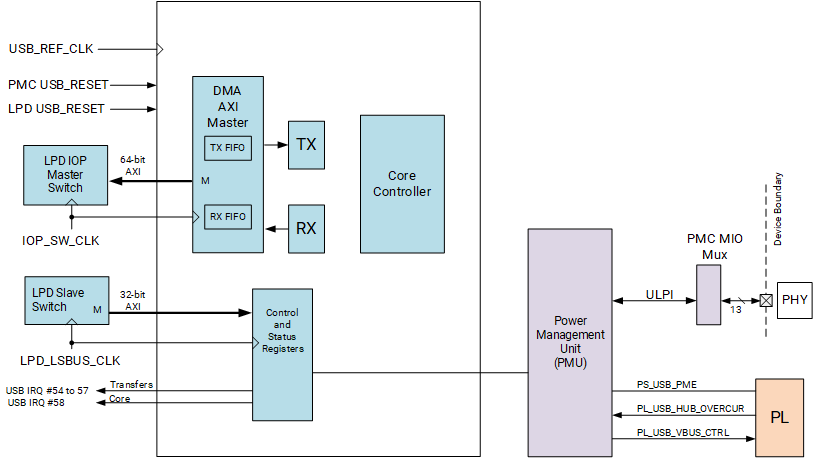
\includegraphics[width=\textwidth]{img/high_level_block_diagr.png}
\caption{Example of high-level block diagram.}\label{fig:example}
\end{figure}

In Figure \ref{fig:example}, DMA stands for Direct Access Memory, LPD indicates ... and so on. Remember to explain any symbols and/or terms and/or acronyms in figures and tables that have not been explicitly explained previously. Remember also to define each acronym before its usage!!!